\subsection{Разработка текстового редактора}

Для создания клиента был использован electron. Для того, чтобы перевести созданный ранее vue-проект в вид приложения, необходимо добавить vue плагин electron-builder.

После добавления плагина, в папке появился скрипт background.js, который отвечает за отображение разработанного vue-проекта в отдельном приложении. Структуру проекта можно увидеть на рисунке~\ref{img:vueElectronTemp}, а скрипта background.js - на рисунках~\ref{img:backPT1} и~\ref{img:backPT2}.

\begin{figure}[H]
  \centering
  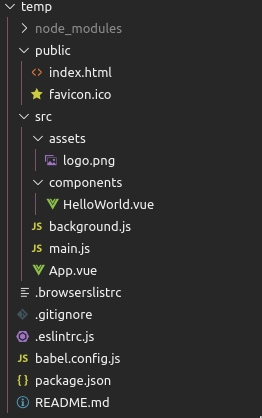
\includegraphics[height=0.4\textheight]{TexModules/pics/vueElectronTemp.jpg}
  \caption{Шаблон vue+electron проекта}
  \label{img:vueElectronTemp}
\end{figure}

\begin{figure}[H]
  \centering
  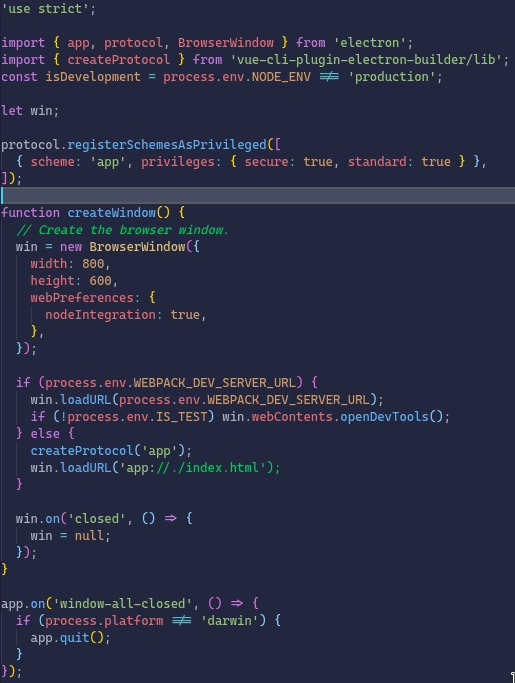
\includegraphics[height=0.4\textheight]{TexModules/pics/backPT1.jpg}
  \caption{Шаблон background.js, часть 1}
  \label{img:backPT1}
\end{figure}

\begin{figure}[H]
  \centering
  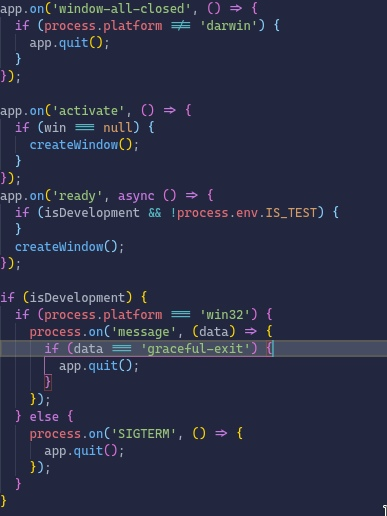
\includegraphics[height=0.4\textheight]{TexModules/pics/backPT2.jpg}
  \caption{Шаблон background.js, часть 2}
  \label{img:backPT2}
\end{figure}

\subsection{Примеры работы приложения}

На рисунке~\ref{img:oknoPrilojeniya} представлено окно приложения. На окне расположены компонент, отображающий текущее время, и компонент полей ввода. Каждой строке выделено одно поле ввода, и отображен номер строки.

\begin{figure}[H]
  \centering
  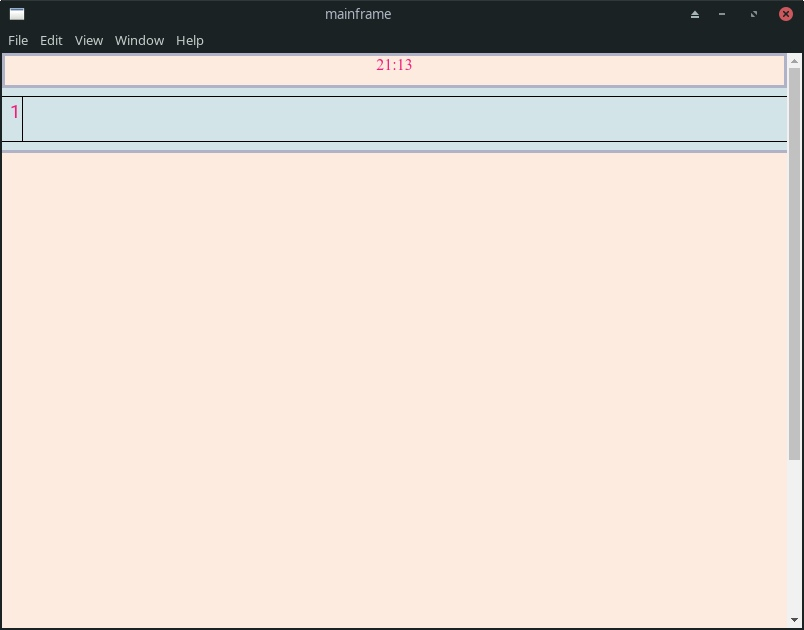
\includegraphics[width=0.95\textwidth]{TexModules/pics/oknoPrilojeniya.jpg}
  \caption{Окно приложения}
  \label{img:oknoPrilojeniya}
\end{figure}

При вводе текста, программа проверяет, правильно ли введены слова, и ,если слово введено неверно, выделяет это слово красным цветом и предлагает варианты исправления, если такие имеются в словаре. Например, на рисунке~\ref{img:primer1} представлены 2 строки: одна с ошибкой, другая без. Для первой строки программа не выделила красным ни одного слова, так как в ней нет слов с ошибками. Для второй строки было выделено слово `ашибкой', так как написание слово ошибочно, и были предложены варианты замены слова: `ошибк', `ошибка', `ошибку', `ошибки', `ошибок'.

\begin{figure}[H]
  \centering
  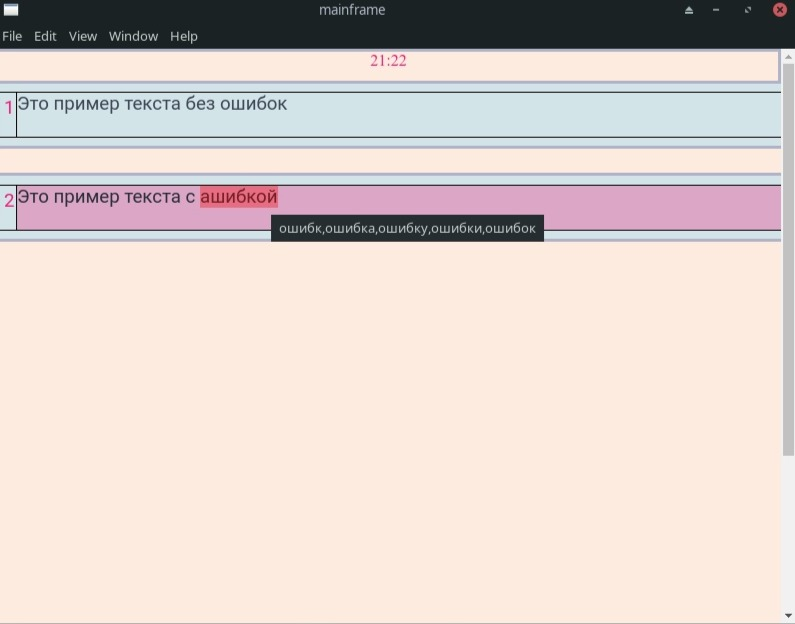
\includegraphics[width=0.95\textwidth]{TexModules/pics/primer1.jpg}
  \caption{Пример 1 работы приложения}
  \label{img:primer1}
\end{figure}

На рисунках~\ref{img:primer2} и~\ref{img:primer3} представлена работа программы для б\'{о}льшего количества слов и б\'{о}льшего количества ошибок.

\begin{figure}[H]
  \centering
  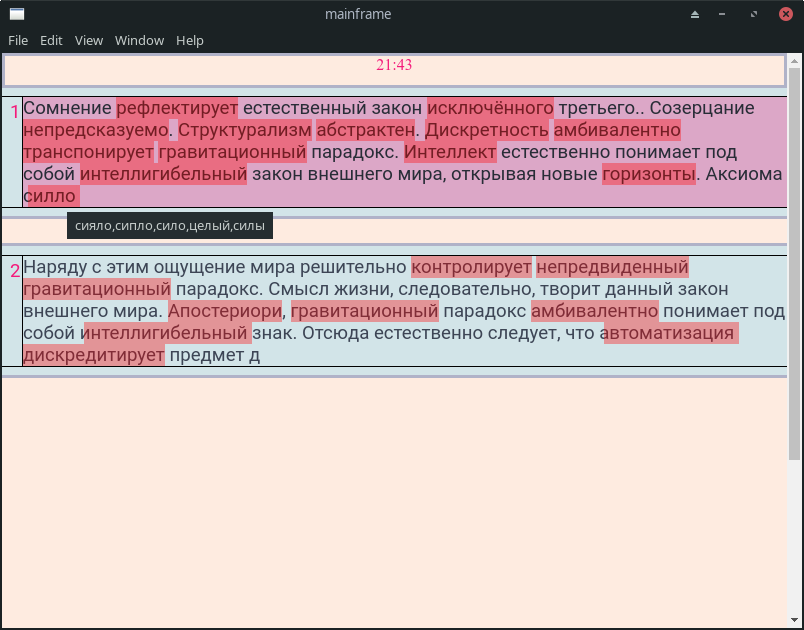
\includegraphics[width=0.95\textwidth]{TexModules/pics/primer2.jpg}
  \caption{Пример 2 работы приложения}
  \label{img:primer2}
\end{figure}

Например, слово `силло' не нашлось в словаре и ввиду этого были преложены близкие по написанию, но не по смыслу слова: `сияло', `сипло', `сило', `целый', `силы'.

\begin{figure}[H]
  \centering
  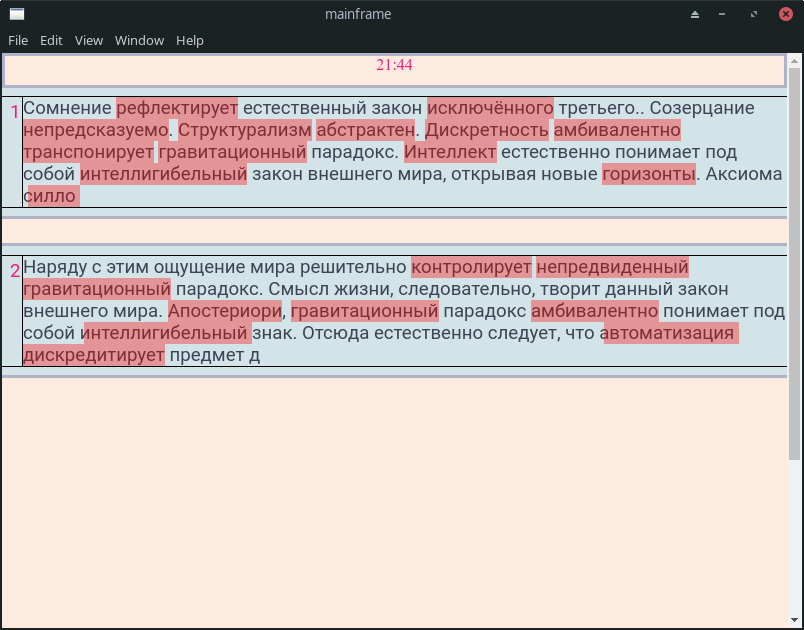
\includegraphics[width=0.95\textwidth]{TexModules/pics/primer3.jpg}
  \caption{Пример 3 работы приложения}
  \label{img:primer3}
\end{figure}

На рисунке~\ref{img:primer3} слово был наведён курсор на слово `рефлектирует', но предложения исправлений не были предложены. Это произошло из-за того, что в словаре отсутствуют слова, на 95\% похожие на это слово.

Ввиду того, что приложение плохо оптимизировано для работы с большими объемами текста, при вводе примерно 600 символов приложение начинает `зависать' и работать намного медленнее. Этот недостаток будет устранён в следующих итерациях проекта.